\documentclass[12pt, a4paper, oneside]{report}
\usepackage[top=1.25in, bottom=1.25in, left=1.5in, right=1in]{geometry}
\usepackage{graphicx}
\usepackage{titlesec}
\usepackage{titletoc}
\usepackage{fancyhdr}
\usepackage{setspace}
\usepackage{times} % Times New Roman font
\usepackage[nottoc]{tocbibind} % Add bibliography to TOC
\usepackage[english]{babel}
\usepackage{amsmath}
\usepackage{amsfonts}
\usepackage{amssymb}
\usepackage{multirow}
\usepackage{tikz}
\usepackage{eso-pic}
\usepackage{array}
\usepackage{longtable}
\usepackage{hyperref}
\usepackage{ragged2e}
\usepackage{booktabs} % Required for \toprule, \midrule, \bottomrule
\usepackage{tabularx} % Optional for better table formatting
\usepackage{enumitem}   % Required for custom enumerate labels
\usepackage{pifont}     % For special symbols (▪)
\usepackage{pgfplots}
\pgfplotsset{compat=1.18}
\usepackage{amssymb}    % For mathematical symbols

\usepackage{lscape}       % For landscape pages
\usepackage{afterpage}    % For page-specific changes
\usepackage{pdflscape}    % Better PDF landscape support

\setlength{\parindent}{1.5em} % Enable and set indent
%\usepackage{parskip} % <- Make sure this is commented out
\usepackage{times}
\renewcommand{\bibname}{References} % Place before 
\onehalfspacing
\setlength{\parindent}{0.5in}

% Chapter formatting
\titleformat{\chapter}[display]
{\normalfont\Large\bfseries\centering}{\chaptertitlename\ \thechapter}{20pt}{\Huge}

% Section formatting
\titleformat{\section}
{\normalfont\large\bfseries}{\thesection}{1em}{}

% Header and footer setup
%\pagestyle{fancy}
%\fancyhf{}
%\fancyhead[LE,RO]{\thepage}
%\fancyhead[RE]{\leftmark}
%\fancyhead[LO]{\rightmark}
%\renewcommand{\headrulewidth}{0.5pt}

% Front matter page numbering (roman)
\newcommand{\frontmatter}{
	\pagenumbering{roman}
	\setcounter{page}{1}
}

% Main matter page numbering (arabic)
\newcommand{\mainmatter}{
	\pagenumbering{arabic}
	\setcounter{page}{1}
} 


\begin{document}	
	
	
\newgeometry{top=1cm, bottom=1.5cm, left=2cm, right=2cm}

	\begin{titlepage}
		\centering			
			
\includegraphics[width=\textwidth]{vppcoe_it_logo.png}			
			\vspace{0.1em}
					
		% === Title ===
		{\Large \textbf{A}}\\[0.5em]
		{\Large \textbf{Major Project Report}}\\[0.5em]		
		{\Large \textbf{on}}\\[1em]
		
		{\LARGE \textbf{Your Title of Project}}\\[1em]
		
		\setstretch{1.3}
		\noindent
		\large{Submitted in partial fulfillment of the requirement for the degree of \\			
			\textbf{Bachelor of Engineering} \\
			Information Technology Semester – VII}\\[1em]
	
		
		\textbf{By}\\ [0.4em]
		Student 1 Name  Roll No \\
		Student21 Name  Roll No \\
		Student 3 Name  Roll No \\
		Student 4 Name  Roll No \\ [0.5em]
		
		\textbf{Under the guidance of}\\
		\textbf{Prof. Your Project Guide  Name}\\[0.7em]
		
		
		Department of Information Technology\\ [0.5em]
		Vasantdada Patil Pratishthan's College of Engineering \& Visual Arts\\ [0.5em]
		% === Department Logo ===
		
\includegraphics[width=0.15\textwidth]{dept_logo.png}\\
		
		
		Vasantdada Patil Educational Complex, Eastern Express Highway, Near Everard Nagar, Sion- Chunabhatti, Mumbai – 400022.\\[0.5em]
		
		{\Large \textbf{University of Mumbai}}\\[0.7em]
		
		{\Large \textbf{2026--27}}
		
	\end{titlepage}	
\restoregeometry
 
	\thispagestyle{empty}
	\newpage
	% === CERTIFICATE PAGE ===

\begin{center}
	
\includegraphics[width=\textwidth]{vppcoe_it_logo.png}
	\newline \\
	\vspace{2em}
	\textbf{\Large CERTIFICATE} \\[2em]
\end{center}

	
	This is to certify that the project entitled \textbf{“Write your project title here”} is bonafide work of Student 1 Name (Roll No), Student 2 Name (Roll No),
	Student31 Name (Roll No), Student 4 Name (Roll No), submitted to University of Mumbai in partial fulfillment of requirement for the award of degree of “Bachelor of Engineering in
	Information Technology Semester VII. \\


\vspace{6em}

\vspace{5em}
\begin{center}
	\textbf{Prof. Your Project Guide Name} \\
	Project Guide
\end{center}

\vspace{10em}

\noindent
\makebox[\textwidth][s]{%
	\textbf{Dr. Pradip Mane}%
	\hfill%
	\textbf{Dr. Alam N. Shaikh }%
}
%Guide
\noindent
\makebox[\textwidth][s]{%
	Head of Department
	\hfill%
	Principal
}



 
	\thispagestyle{empty}
	\newpage
	% === DECLARATION PAGE ===
\begin{center}
	
\includegraphics[width=\textwidth]{vppcoe_it_logo.png}
	\newline \\		
	\vspace*{1cm}
	\textbf{\Large Project Report Approval for B. E.} \\[2em]
\end{center}

This project report entitled \textbf{“Insert your project title here”} byStudent 1 Name (Roll No), Student 2 Name (Roll No),Student 3 Name (Roll No), Student 4 Name (Roll No), is approved for the degree of Bachelor of Engineering in Information Technology. \\ \\

\vspace{8em}
\begin{center}
\textbf{Examiners} \\[1cm]
\end{center}
\begin{flushright}
	
	1.\ \underline{\hspace{8cm}} \\[2cm]
	2.\ \underline{\hspace{8cm}}
\end{flushright}
\vspace{4em}
Date: 
\vspace{2em} \\
Place: 
	\thispagestyle{empty}
	\newpage
	% === DECLARATION PAGE ===

\begin{center}
	
\includegraphics[width=\textwidth]{vppcoe_it_logo.png}
	\newline \\
	\vspace{2em}	
	\textbf{\Large DECLARATION} \\[2em]
\end{center}

We declare that this written thesis submission represents the work done based on our and/or others’ ideas with adequately cited and referenced the original sources. We also declare that we have adhered to all principles of intellectual property, academic honesty, and integrity as we have not misinterpreted, fabricated, or falsified any idea/data/fact/source or original work/matter in our submission.

We understand that any violation of the above will be cause for disciplinary action by the college and may evoke penal action from the sources which have not been
properly cited or from whom proper permission is not sought. \\

\vspace{4em}
\begin{flushright}
	\noindent 1.  Student 1 Name  Roll No \underline{\hspace{4cm}} \\[2em]
	\noindent 2.  Student 2 Name  Roll No \underline{\hspace{4cm}}\\[2em]
	\noindent 3.  Student 3 Name  Roll No \underline{\hspace{4cm}}\\[2em]
	\noindent 4.  Student 4 Name  Roll No \underline{\hspace{4cm}}\\[2em]
\end{flushright}
\vspace{3em}
Date: 
\vspace{2em} \\
Place: 
	\thispagestyle{empty}
	\newpage
	% === ACKNOWLEDGEMENT PAGE ===

\begin{center}
	
\includegraphics[width=\textwidth]{vppcoe_it_logo.png}
	\newline \\
	\vspace{2em}	
	\textbf{\Large ACKNOWLEDGEMENT} \\[2em]
\end{center}

We the students from Vasantdada Patil Pratishthan’s College of Engineering and Visual Arts, Mumbai of Final Year Engineering in the department of ‘Information Technology’
have great pleasure in presenting our efforts of developing the project named as \textbf{“Insert your project title”}.\\

We would like to express our heartfelt gratitude to \textbf{Dr. Pradip Mane}, Head of Department, for providing us with inspiration, valuable guidance, and timely suggestions throughout our Mini project journey.\\

Our immense appreciation also goes to our esteemed Guide \textbf{Prof. Your Guide Name} for his unwavering support and the opportunity he provided us to undertake this challenging project have been truly invaluable. This experience not only allowed us to conduct extensive project work but also exposed us to a wealth of new knowledge for which we are genuinely thankful. Also, we would also like to express our gratitude to the Major Project Coordinator, \textbf{Prof Priyanka Manke} for her insightful inputs.
  \\

\vspace{4em}
\begin{flushright}
	\noindent 1.  Student 1 Name  Roll No \\[2em]
	\noindent 2.  Student 2 Name  Roll No \\[2em]
	\noindent 3.  Student 3 Name  Roll No \\[2em]
	\noindent 4.  Student 4 Name  Roll No\\[2em]
\end{flushright}

	\thispagestyle{empty}
	
	
	% Front Matter Content
	\frontmatter
	% Abstract
	% ABSRACT PAGE
\chapter*{Abstract}
\begin{spacing}{1.5}
	
The Abstract serves as a condensed version of your entire project. According to the syllabus, it must reflect the process of identifying a need and converting it into a problem statement. It acts as a standalone summary that allows a reader to understand the essence of your Web-Based ML project without reading the full document.

Abstract Length Guidelines
For a Mini Project of this scale, the abstract should typically be between 250 to 300 words. It should fit on a single page and be written as a single, continuous paragraph or a few short, dense paragraphs.

Detailed Guidelines for Writing the Abstract
To meet the assessment criteria for clarity and societal impact, follow this structural flow:

1. Context and Motivation (2–3 sentences)
Start with the domain (Web + ML).
State the societal or research need identified during your survey.

Example: "With the rise of digital health, there is a significant need for accessible diagnostic tools for rural populations..."

2. Problem Statement (1–2 sentences)

Clearly define the technical problem you are solving.

Mention the specific gap identified in existing systems.

3. Proposed Solution and Methodology (3–4 sentences)

Identify the specific ML algorithms and web technologies used.

Briefly mention the data source and the "best possible solution" selected.

Example: "This project proposes a Flask-based web application integrated with a Random Forest model trained on the XYZ dataset..."

4. Results and Validation (2–3 sentences)

Highlight the "full functioning of the working model".

Mention key performance metrics (accuracy, efficiency) obtained through simulations or testing.

5. Impact and Conclusion (1–2 sentences)

State how the project achieves "sustainable development" or maps to an SDG.

Summarize the cost-effectiveness and societal value of the final product.

Abstract "Checklist" for Students
No Citations: Do not include references (e.g., [1]) in the abstract.
No Figures/Tables: Keep it strictly text-based.

Past Tense: Since the abstract summarizes work already done, use the past tense (e.g., "The model was trained..." or "The survey was conducted...").

Keywords: Include 4–6 keywords at the bottom (e.g., Machine Learning, Web Development, SDG 3, Predictive Modeling).
\newline	\\
\textbf{Keywords:} AI,  Machine Learning, (include atleast five keywords) 	
	
\end{spacing}
	
	% Table of Contents
	\renewcommand{\contentsname}{Table of Contents}
	\tableofcontents
	
	% List of Figures
	\listoffigures
	
	% List of Tables
	\listoftables
	
	%Acronyms
	\begin{flushright}
	
\end{flushright}\chapter*{Acronyms}
\begin{tabbing}
	xx\=xxxxxxxxxxxxxxxxx\=xxxxxxxxxxxxxxxxxxxxxxxxxxxxxxxxxxxxxxxxxxxxxxxxx\=xxxxxxxxxx\kill
	\>ML  \>  Machine Learning\\
	\>DL  \>  Deep Learning\\
	\>SVM  \>  Support Vector Machine\\
	\>DT  \>  Decesion Tree\\
	\>RF  \>  Random Forest\\	
	 \>CNN  \> Convolutional Neural Networks\\
	 \>NB  \> Naive Bayes\\
	 \>LR  \> Logistic regression\\
	 
	  Replace the aabove acronyms with acronymsused in your project
	 	
\end{tabbing}
	
	\newpage
	% Main Content
	\mainmatter
	
	% Chapter 1: Introduction
	%INTRODUCTION PAGE

\chapter{Introduction}

This project emphasizes the application of engineering fundamentals to solve real-world challenges. The primary goal of this initiative is to leverage the synergy between Machine Learning and Web Development to address specific societal or research needs identified through an extensive survey. By converting these needs into a well-defined technical problem, the project strives to develop a functional working model that is not only innovative but also aligned with Sustainable Development Goals (SDGs). This introductory chapter provides the foundational context for the study, detailing the background, motivation, and technical objectives that guided the development and implementation of the proposed solution.

\section{Background}

Briefly describe the evolution of Web Development and its transition from static pages to intelligent, data-driven platforms. 

Introduce Machine Learning as the core logic that enables the system to learn from data and make predictions or decisions.

Explain the synergy between the two: why a web interface is the best delivery mechanism for making an ML model accessible to end-users.

 That is clustering of the nearest approximate value. the 42\% who reported no physical or chronic conditions as shown in Figure \ref{fig:Prevalence}.  public health concerns  \cite{b2}.

\begin{figure}[h]
	\centering
	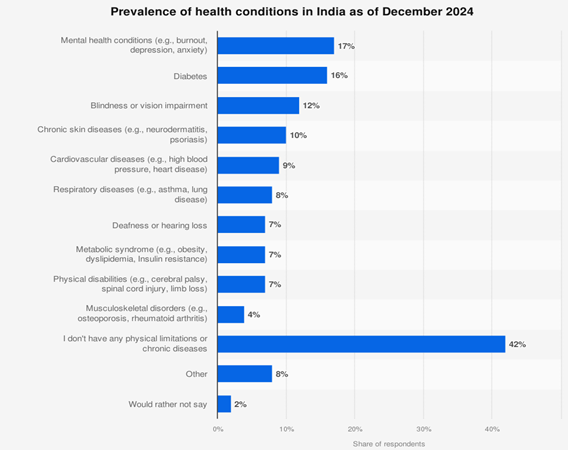
\includegraphics[width=\textwidth]{prevalence.png}
	\caption{Prevalence of health conditions in India as of December 2024 \cite{b2}}
	\label{fig:Prevalence}
\end{figure}

\section{Motivation}
Here, you explain the "Why" behind your project choice.
Detail the specific societal or research needs you discovered during your initial survey.

Discuss the current challenges or pain points faced by the target audience.

Mention your desire to apply engineering fundamentals to solve a real-world problem rather than a purely theoretical one.
\begin{itemize}
	\item Time taken to hire a person. 
	\item Confusion of selecting whom to select.
	\item To improve the tedious process.	
\end{itemize}

\section{Problem Definition}

This is a precise, technical translation of the motivation.
Statement of Need: Summarize the gap identified in Section .

Technical Problem: Convert that need into a technical challenge (e.g., "Designing a robust CNN-based web application to detect crop diseases with an accuracy of over 90\% in real-time").

Scope: Explicitly state what the project will cover and what it will not, ensuring the project is feasible within the semester timeline.

\section{Aim and Objectives of the project}

\subsection{Aim}

Our aim is to help the HR round go more smoothly and efficiently so that a person’s skill can be predicted beforehand without wasting much of the time of the HR. also to sort the resumes according to the requirements of the organizations. And to take the current CV ranking system to an advanced level.

\subsection{Objectives}

Specific goals, including the development of a functional working model. List the "What" of your project in measurable terms.
\begin{itemize}
	\item Identify and pre-process a domain-specific dataset. 
	\item TDesign and train a specific Machine Learning algorithm.
	\item Develop a functional working model with a user-friendly web interface.
	\item Evaluate the model using standard metrics like accuracy, precision, or cost-effectiveness.	
\end{itemize}

\section{Scope of the Project} 

IT sector has largest recruiting sector. Our proposed system is initially concerned with IT companies and to recruit the right candidate with perfect skills and technical skills. IT recruitment is in bulk so to reduce the manual work and make sure the intake is of the right candidate. It is also applicable for different jobs and profession.

\section{Sustainable Development Goal (SDG) Mapping} 
This is a mandatory requirement for analyzing the impact of your solution.
Identify the Goal: Specify the exact UN SDG number and title (e.g., Goal 3: Good Health and Well-being).

Impact Analysis: Provide a detailed explanation of how your specific ML solution contributes to this goal.

Environmental Context: Briefly discuss the sustainability of your solution—how it uses resources efficiently or promotes environmental welfare.\\\\


\section{Organization of the Report} 
The remainder of this report is organized into five subsequent chapters to provide a comprehensive overview of the project’s lifecycle. Chapter 2 presents a detailed literature survey of existing systems and identifies the research gap that justifies the need for this work. Chapter 3 outlines the methodology, system architecture, and project planning, including the Gantt chart for implementation. Chapter 4 details the core implementation phase, covering dataset pre-processing, Machine Learning model development, and the integration of the web-based interface. Chapter 5 provides a demonstration of the working prototype along with an analysis of experimental results and performance metrics. Finally, Chapter 6 concludes the report by summarizing the project's achievements, individual contributions, and potential directions for future research in line with the goals of life-long learning.

	
	% Chapter 2: Literature Review
	%LITERATURE REVIEW

\chapter{Literature Survey}

In Chapter 2, students demonstrate the "quality of survey/need identification" and "clarity of problem definition based on need"  as required by the syllabus. This chapter provides the scholarly grounding for the project.

\section{Existing Systems}

This section is an analysis of current solutions based on the survey results students are required to conduct.

Current Landscape: Describe the popular web applications or software tools currently used to address the identified problem.

Methodology of Current Tools: Explain the technologies or Machine Learning models these existing systems typically employ.

Functionality: Detail the features provided by these systems and how they serve the current user base.

\section{Comparative Study}
This section summarizes various methods found in research to "inculcate the process of self-learning and research".

Algorithm Comparison: Create a table comparing different ML algorithms (e.g., SVM vs. Random Forest vs. CNN) used in previous research papers.

Performance Metrics: Compare results from different theoretical or experimental simulations found in the literature, such as accuracy, latency, or resource consumption.

Technical Constraints: Discuss the hardware and software limitations associated with each researched method.

Studies in this field examine various aspects, including data collection, feature extraction, model training, and performance evaluation, with each study presenting unique insights into the detection process. Table \ref{tab:depression_ML} highlights their datasets, methods, and results for quick comparison.

\begin{table}[htbp]
	\centering
	\caption{Summary of depression detection using machine learning techniques}
	\label{tab:depression_ML}
	\small
	\begin{tabular}{
			>{\RaggedRight}p{0.6cm}    % Ref. (narrow)
			>{\RaggedRight}p{2cm}  % Authors (wider)
			>{\RaggedRight}p{0.6cm}  % Year		
			>{\RaggedRight}p{5cm}    % Results
			>{\RaggedRight}p{5cm}    % Limitations
		}
		\toprule
		\textbf{Ref.} & \textbf{Author(s)} & \textbf{Year} & \textbf{Results} & \textbf{Limitations} \\
		\midrule
		\cite{b1} & R. Chiong et al. & 2021 & 98\% accuracy with Gradient Boosting; Combines lexical and content features for robustness, strong feature mix, handles uneven data well, beats baseline results. & Needs labelled data, Does not work for other languages, focuses only on Twitter, uses default settings, manual feature design. \\
		\hline
		\addlinespace
		\cite{b2} & M. S. Liaw et al. & 2022 & 82\% F1-score; User engagement metrics improve detection, better user behavior insights & Data privacy concerns; Network features not significant, Some text incomplete or unclear \\
		\bottomrule
		\hline
	\end{tabular}
\end{table}

\section{Research Gap}

This is the most critical part of the survey, where students identify why a new solution is required to fulfill a societal or research need.

\begin{itemize}
	\item Limitations of Existing Systems: Point out specific shortcomings in current solutions, such as high cost, low accuracy, or lack of a user-friendly web interface.
	\item Unmet Needs: Highlight the specific societal or research requirements that remain unaddressed by the literature surveyed.
	\item Justification for New Project: Clearly state how the proposed "Mini Project - 2 B" will fill these gaps using domain-specific skill sets and engineering fundamentals.	
\end{itemize}



	
	% Chapter 3: Research Objectives
	% RESEARCH OBJECTIVES

\chapter{Design and Planning}

In Chapter 3, students translate their research into a concrete engineering plan. This chapter directly addresses the syllabus requirements for "proposing multiple solutions and selecting the best possible solution" and "demonstrating project management principles".

\section{Proposed Solution}	
This section describes the "best possible solution" selected for the underline problem.

Core Approach: Detail the specific Machine Learning algorithm chosen (e.g., Random Forest, CNN, or LSTM) and why it is the most suitable for the identified societal problem.

Web Integration Strategy: Explain how the ML model will be served via the web (e.g., using Flask, Django, or FastAPI).

Innovation: Highlight the "innovativeness in solutions" as per the assessment criteria.

\section{System Architecture}	  
This provides a visual and technical roadmap of the "working model". Our system follows the three tier architecture. First tier consist of GUI, followed by Processing block and the Database.

\subsection{GUI (Graphical User Interface)}
In our project GUI deals with the interface for the user where the user will have to register and then login give the skill test and submit his resume in any format (Pdf, doc, docs, etc.)

\subsection{Processing block}
This is the block where the actual processing of our project is done. This block will connect the database and the GUI .i.e. it acts as a connector as well as communicator which connects the database and helps in transfer of data between the GUI and the database. Its main function will be to take input from the uploaded CV of the candidate.

\subsection{Databas:}
Database tier is used for the data storage. This contains all the data that is need for the processing and string data of the project. The data in this tier is related to the student information gathered from his/her CV.

\section{Design}

Include the UML Diagram as per requirement of your project
\subsection{Use case Diagram}

\subsection{Activity Diagram/ Sequence Diagram}

\subsection{Data Flow Diagram}

\section{Algorithm}
Explain the algorithms used in your project.
\subsection{K- Means Algorithm}
The Lloyd's algorithm, mostly known as k-means algorithm, is used to solve the k-means clustering problem and works as follows. First, decide the number of cluster:
Step 1: Initialize the center of the clusters
Step 2:.Attribute the closest cluster to each data point
Step 3: Set the position of each cluster to the mean of all data points belonging to that cluster Step 4 : Repeat steps 2-3 until convergence


\section{Component Selection}
This section documents the "system selection and cost analysis" required by the project.

Software Selection: Justify the choice of programming languages (e.g., Python), libraries (e.g., Scikit-learn), and web frameworks based on "engineering fundamentals".

Hardware Requirements: List the computational resources needed for training the model and hosting the web application.

Cost Analysis: Provide a detailed breakdown of costs (if any) to ensure "cost effectiveness," a key assessment criterion.

\section{Implementation Plan}
Weekly activity breakdown using a Gantt, PERT, or CPM chart.
Students must demonstrate "project management principles" by organizing their work into a schedule.

Weekly Activity Breakdown: Each group must provide an "implementation plan in the form of Gantt/PERT/CPM chart".

Milestones: Map key activities—such as "identification of need," "building prototype," and "testing"—to specific weeks of the semester.

Self-Learning Progress: Align the plan with the "log book" entries to record weekly work progress for verification by the project guide.


	
	% Chapter 4:Implementation and Testing
	
\chapter{Implementation and Testing}

This chapter documents the construction of the working prototype and the tests applied to it. It explains how the proposed architecture was converted into a functioning gateway: the dataset used for training, the machine-learning models and their configuration, the web interface, and the evaluation carried out to validate the result.

\section{Data Collection and Pre-processing}

\textbf{Dataset Identification.} The dataset was generated specifically for this project by the custom generator \texttt{scripts/generate\_dataset.py}, which produces realistic HTTP requests (method, URL, headers, body and per-client traffic statistics). Public intrusion-detection corpora were not used because they contain raw network packets rather than the application-layer requests inspected by the gateway.

\textbf{Data Description.} The cleaned file \texttt{dataset/ml\_dataset\_fixed.csv} contains 499,755 records with 20 model features, a binary label and an attack category. The label distribution is 299,755 benign records (59.98\%) and 200,000 attack records (40.02\%) across thirteen attack categories, the largest being SQL injection (29,966), cross-site scripting (29,899), prompt injection (20,261) and path traversal (19,848). The features combine continuous measurements such as URL length, URL entropy, body length, header count, requests per minute and error rate with binary pattern flags for SQL, JavaScript, traversal, command-injection, XXE and prompt-injection content.

\textbf{Pre-processing Steps.} Two label-derived columns (\texttt{risk\_score} and \texttt{severity}) were removed because they encode the answer and would leak it into the model; earlier experiments that retained them reached a deceptively perfect accuracy of 1.0000. The behavioural columns were then re-sampled so that benign and attack records overlap realistically, removing the artificial separation that had produced 0.9988 accuracy. The dataset contains no duplicate rows and no missing values among the twenty model features. Feature scaling uses \texttt{StandardScaler}, fitted on the training partition only.

\textbf{Data Splitting.} The data was divided 80:20 into training and testing sets using stratified sampling with a fixed random seed of 42, giving 399,804 training records and 99,951 test records while preserving the class ratio in both partitions. Stratification keeps the minority attack classes represented on both sides, and the fixed seed makes every later experiment reproducible.

\section{ML Model Development}

\textbf{Algorithm Selection.} Nine supervised classifiers were trained on the same split and compared: multi-layer perceptron, gradient boosting, decision tree, random forest, k-nearest neighbours, logistic regression, linear SVM, AdaBoost and extra trees. Random Forest was selected for deployment inside the gateway. Although the multi-layer perceptron achieved the highest raw accuracy (0.9084), Random Forest was preferred because it produced the highest precision among the leading models (0.9906), the smallest gap between training and testing accuracy (0.0004) and an AUC of 0.9377. In a gateway a false positive blocks a legitimate user, so precision is weighted above recall; Random Forest also returns deterministic predictions, per-feature importances for the explanation panel, and low inference cost on every request.

A second, unsupervised model, Isolation Forest, complements it. This model is trained only to recognise normal traffic and therefore does not require attack labels, which allows it to flag request shapes that were absent from the training data. Its threshold is set at the fifth percentile of the training anomaly scores, which limits it to approximately 95\% specificity. Measured precision is 0.9996 and specificity 0.99997, with a lower recall of 0.121, so it functions as a safety net contributing a capped number of risk points rather than as a primary detector.

\textbf{Training Process.} Training was performed offline in Python 3.12 using scikit-learn on a Windows workstation. The cleaned dataset was scaled with \texttt{StandardScaler} fitted on the training partition, after which every classifier was fitted with a fixed random seed. The artifacts used by the gateway are the exported Random Forest model and its scaler (\texttt{models/aegis\_model.pkl} and \texttt{models/scaler.pkl}); the gateway reads no dataset at run time. Five-fold cross-validation on a 30,000-record subset produced a mean accuracy of 0.8281 with a standard deviation of 0.0023 for Random Forest, confirming that the result does not depend on a single favourable split.

\textbf{Model Optimization.} Three optimisation steps were applied. First, the label-derived columns \texttt{risk\_score} and \texttt{severity} were removed, eliminating the leakage that had produced an accuracy of 1.0000. Second, the behavioural features were re-sampled so that benign and attack records overlap, which removed the remaining artificial separation that had produced 0.9988 accuracy. Third, the model was regularised with a maximum depth of 12, a minimum of 5 samples per leaf and balanced class weights, which kept the training and testing accuracies within 0.0004 of each other. On the held-out test partition of 99,951 records the final model reached an accuracy of 0.8847, precision of 0.9906, recall of 0.7186, F1 of 0.8330 and AUC of 0.9377, with 274 false positives among 59,951 benign records.

Table \ref{tab:hyper_parameters} shows the hyperparameter values used for the deployed models.

\begin{table}[htbp]
	\centering
	\caption{Hyperparameters}
	\label{tab:hyper_parameters}
	\small
	\begin{tabular}{
			>{\RaggedRight}p{6.0cm}
			>{\RaggedRight}p{6.0cm}
		}
		\toprule
		\textbf{Parameters} & \textbf{Values} \\
		\midrule
		Classifier & Random Forest (scikit-learn) \\
		\hline
		\addlinespace
		Number of trees & 100 \\
		\hline
		\addlinespace
		Maximum depth & 12 \\
		\hline
		\addlinespace
		Minimum samples per leaf & 5 \\
		\hline
		\addlinespace
		Class weight & Balanced \\
		\hline
		\addlinespace
		Feature scaling & StandardScaler (zero mean, unit variance) \\
		\hline
		\addlinespace
		Train/test ratio & 80:20, stratified \\
		\hline
		\addlinespace
		Random seed & 42 \\
		\hline
		\addlinespace
		Isolation Forest trees & 200 \\
		\hline
		\addlinespace
		Isolation Forest contamination & 0.4002 \\
		\hline
		\addlinespace
		Anomaly threshold & 5th percentile of training scores ($-0.1053$) \\
		\bottomrule
	\end{tabular}
\end{table}

\section{Web Interface Development}

\textbf{Frontend Design.} The administrative interface is a single-page dashboard written in plain HTML, CSS and JavaScript (\texttt{gateway/static/index.html}) with no build step. It presents summary tiles for total, blocked, challenged and forwarded requests; a live request table showing method, path, client address, risk score, action and status; category and text filters; and a detail dialog containing stacked contribution bars for the rule, machine-learning, isolation-forest, behavioural and threat-intelligence components, the leading explanation reasons, a counterfactual suggestion, the matched rule signatures and the twenty extracted feature values. Separate panels manage blocked addresses, source reputation, the application profile and model information, while setup fields control the target URL and the operating mode. The request table refreshes every 2.5 seconds and the blocked-address list every 7 seconds.

\textbf{Backend Integration.} The interface is served by the same FastAPI application that performs request inspection, so no additional web server is required. The application exposes a JSON interface comprising \texttt{/api/health}, \texttt{/api/target}, \texttt{/api/config}, \texttt{/api/logs}, \texttt{/api/stats}, \texttt{/api/model}, \texttt{/api/blocked}, \texttt{/api/unblock}, \texttt{/api/reputation}, \texttt{/api/challenge}, \texttt{/api/profile} and \texttt{/api/reset}, through which the dashboard reads state and applies administrative changes.

\textbf{API/Service Flow.} Every inspected request is written to an in-memory log as a complete record containing the score, its components, the decision, the explanation and a summary of the response returned to the client. The browser polls \texttt{/api/logs} and \texttt{/api/stats} and renders the returned records; selecting a row displays that record in the detail dialog. Administrative actions such as unblocking an address, changing the target, running the profiler or resetting the log are POST requests whose effect appears on the following poll. When a request is challenged, the gateway returns HTTP 401 with an arithmetic question; the browser submits the answer to \texttt{/api/challenge}, which issues the clearance cookie, and the original request is repeated and then forwarded.

\section{Testing}

Five groups of tests were used to validate the implementation.

\begin{enumerate}
	\item \textbf{Pipeline unit gate} (\texttt{gateway/test\_pipeline.py}): verifies that the live feature vector matches the training column order, that benign requests score below the challenge threshold, that attack requests reach or exceed it, that the arithmetic challenge can be issued, verified and converted into a clearance, and that blocklist escalation works. Result: passed with exit code 0.
	\item \textbf{End-to-end HTTP tests} (\texttt{gateway/test\_phases.py}): 44 checks across phases 5--10 covering service health, dashboard availability, completeness of logged records, direct-versus-gateway vulnerability comparison, application discovery, decoy and honeytoken behaviour, all three decision bands, double-encoded payloads and malicious-source blocking. Result: 44/44 passed.
	\item \textbf{Signature accuracy} (\texttt{tools/rule\_check.py}): 13 attack payloads must be detected and 17 benign queries must not be flagged. Result: 0 attacks missed, 0 benign queries flagged.
	\item \textbf{Adversarial mutation audit} (\texttt{tools/mutation\_audit.py}): 71 mutated variants of known payloads applying encoding changes, case changes, comment insertion, method changes and header changes. Result: 0 leaks -- every mutation reached at least the challenge band.
	\item \textbf{Model evaluation}: the exported model was evaluated on the held-out test partition of 99,951 records, giving 0.8847 accuracy, 0.9906 precision, 0.7186 recall, 0.8330 F1 and 0.9377 AUC, with 274 false positives out of 59,951 benign records.
\end{enumerate}

Two limitations were measured honestly during adversarial testing. First, two hand-crafted requests were forwarded with risk scores of 7 and 5 because the rule boundary patterns do not recognise an ampersand inside a parameter value or a SQL comment that is not followed by whitespace, while the machine-learning contribution is capped at 30 points, below the 31-point challenge threshold. Second, the clearance cookie is bound to a client address for 600 seconds rather than to the individual request that was solved. Both findings are recorded as future work rather than hidden.

	
	% Chapter 5: Results
	

\chapter{Results and Discussion}

In Chapter 5, students provide evidence of the "full functioning of working model as per stated requirements". This chapter is critical for the "Review 2" assessment, as it validates the "implementation and testing of the solution". 

\section{Working Prototype Demonstration}
Screenshots and descriptions of the functional model. This section serves as the visual proof of the "working model".

Interface Walkthrough: Include high-quality screenshots of the web application’s frontend, including input forms and result displays.

System Functionality: Provide a step-by-step description of how a user interacts with the ML model through the web interface.

Feature Verification: Map each screenshot to the initial "stated requirements" to prove the prototype is fully functional.

User Feedback (if any): Describe how the interface facilitates "societal impact" by being accessible to the target users.

\section{Validation and Inference}
Drawing proper inferences from experimental results or simulations. Students must demonstrate their ability to "draw the proper inferences from available results".

Experimental Results: Present data obtained through "theoretical, experimental, or simulations".

Justification of Results: Provide a "proper justification" for why the model produced specific outputs.

Inference Drawing: Explain what the results mean in the context of the "societal/research needs" identified in Chapter 1.

Comparative Validation: Briefly discuss how these results compare to the "proposed multiple solutions" considered during the design phase.


\section{Performance metrics} 

Accuracy, cost-effectiveness, and efficiency analysis. In this section, we explain the performance metrics used to check the performance of model. These metrices include accuracy, precision, recall, and F1-score. This section quantifies the "excellence" and "efficiency" of the engineering solution.

ML Accuracy: Use standard metrics such as Accuracy, Precision, Recall, and F1-Score to evaluate the "skill sets" applied in model training.

Confusion Matrix: Include a visual representation of the model's classification performance to support "validation with proper justification".

Cost-Effectiveness: Provide an analysis of "cost effectiveness" by comparing the performance gained against the resources/computation used.

System Efficiency: Analyze the "impact of solutions" in terms of response time and resource efficiency for "sustainable development".		
	
	% Chapter 6: Conclusion
	% CONCLUSION

\chapter{Conclusion and Future Work}

In the final chapter, students summarize their findings and reflect on the project management principles and individual growth achieved during the semester. This chapter is essential for demonstrating the "Course Outcomes" related to life-long learning and interpersonal skills.

\section{Conclusion}
This section provides a holistic summary of the "working model" and its alignment with the initial project goals.

Project Summary: Briefly restate the problem and the specific Web-ML solution developed.

Requirement Validation: Explain how the final prototype meets all "stated requirements" and addresses the identified "societal/research needs".

Impact Statement: Summarize the "societal and environmental context" of the project, specifically how it contributes to the mapped Sustainable Development Goals (SDGs).

\section{Future Scope:}
This section demonstrates the "capabilities of self-learning in a group, which leads to life-long learning".

Technical Improvements: Suggest potential enhancements, such as using more advanced ML algorithms, improving UI/UX, or scaling the web infrastructure.

Feature Extension: Identify additional features that could be added to increase the project's "cost effectiveness and societal impact".

Research Directions: Mention how this project could serve as a foundation for further research or a "one-year project" extension in the next semester.
	
	% References
	% REFERENCES

%\chapter*{References}
\renewcommand{\bibname}{References} % Place before

\begin{small}

\begin{thebibliography}{30}
	\bibitem{b1}
		M. E. Durmuşkaya and S. Bayraklı, "Web application firewall based on machine learning models," \textit{PeerJ Comput. Sci.}, vol. 11, e2975, 2025, doi: 10.7717/peerj-cs.2975.
	\bibitem{b2}
		R. Bakır, "UniEmbed: A novel approach to detect XSS and SQL injection attacks leveraging multiple feature fusion with machine learning techniques," \textit{Arab. J. Sci. Eng.}, vol. 50, pp. 15591--15604, 2025, doi: 10.1007/s13369-024-09916-4.
	\bibitem{b3}
		S. S. Ahmed and M. L. Al dabag, "Deployment-oriented multi-embedding machine learning framework for SQL injection detection and prevention in a web application firewall," \textit{Computers}, vol. 15, no. 6, art. 368, 2026, doi: 10.3390/computers15060368.
	\bibitem{b4}
		Y. Zhou, E. Wang, W. Yang, W. Ge, S. Yang, Y. Zhang, W. Qu, and W. Xie, "XSShield: Defending against stored XSS attacks using LLM-based semantic understanding," \textit{Appl. Sci.}, vol. 15, no. 6, art. 3348, 2025, doi: 10.3390/app15063348.
	\bibitem{b5}
		T. I. Korobeinikova and N. V. Kravchuk, "ML-WAF information technology for classification and blocking of injection attacks in a containerized Web environment," \textit{Radiotekhnika}, no. 4(223), pp. 100--110, 2025, doi: 10.30837/rt.2025.4.223.11.
	\bibitem{b6}
		M. T. A. Nguyen, V. Tong, S. B. Souihi, and S. Souihi, "Zero trust: Deep learning and NLP for HTTP anomaly detection in IDS," \textit{IEEE J. Sel. Areas Commun.}, vol. 43, no. 6, pp. 2215--2229, Jun. 2025, doi: 10.1109/JSAC.2025.3560040.
	\bibitem{b7}
		V. Z. Mohale and I. C. Obagbuwa, "Evaluating machine learning-based intrusion detection systems with explainable AI," \textit{Front. Comput. Sci.}, vol. 7, art. 1520741, 2025, doi: 10.3389/fcomp.2025.1520741.
	\bibitem{b8}
		B. Nugraha, A. V. Jnanashree, and T. Bauschert, "A versatile XAI-based framework for efficient and explainable intrusion detection systems," \textit{Ann. Telecommun.}, vol. 80, nos. 11--12, pp. 1095--1120, 2025, doi: 10.1007/s12243-025-01118-9.
	\bibitem{b9}
		F. Ebrahimi, R. Javidan, R. Akbari, and Y. Hosseini, "Intrusion detection in the internet of things using convolutional neural networks: An explainable AI approach," \textit{Cybersecurity}, vol. 8, no. 1, art. 66, 2025, doi: 10.1186/s42400-025-00369-2.
	\bibitem{b10}
		A. E. Muhammad, K.-C. Yow, N. Bačanin-Džakula, and M. A. Khan, "L-XAIDS: A LIME-based eXplainable AI framework for intrusion detection systems," \textit{Cluster Comput.}, vol. 28, no. 10, art. 654, 2025, doi: 10.1007/s10586-025-05326-9.
	\bibitem{b11}
		K. P. Sharma, T. Nagpal, T. Vora, A. Yadav, and M. I. Abdullah, "Interpretable intrusion detection for IoT environments using a self-attention-based explainable AI framework," \textit{Sci. Rep.}, vol. 15, art. 39937, 2025, doi: 10.1038/s41598-025-23750-0.
	\bibitem{b12}
		S. Okada, H. Jmila, K. Akashi, T. Mitsunaga, Y. Sekiya, H. Takase, G. Blanc, and H. Nakamura, "XAI-driven black-box adversarial attacks on network intrusion detectors," \textit{Int. J. Inf. Secur.}, vol. 24, no. 3, art. 103, 2025, doi: 10.1007/s10207-025-01016-0.
	\bibitem{b13}
		S. Ennaji, E. Benkhelifa, and L. V. Mancini, "Vulnerability disclosure through adaptive black-box adversarial attacks in network intrusion detection systems," \textit{Complex Intell. Syst.}, vol. 12, no. 1, art. 18, 2026, doi: 10.1007/s40747-025-02115-0.
	\bibitem{b14}
		W. Yao, H. Peng, Q. Li, and X. Shen, "Modeling realistic adversarial traffic against deep-learning-based intrusion detection system in industrial IoT," \textit{IEEE Internet Things J.}, vol. 12, no. 15, pp. 29540--29554, 2025, doi: 10.1109/JIOT.2025.3568503.
	\bibitem{b15}
		J. Sun and S. Yang, "Adversarial sample generation based on model simulation analysis in intrusion detection systems," \textit{Electronics}, vol. 14, no. 5, art. 870, 2025, doi: 10.3390/electronics14050870.
	\bibitem{b16}
		V. Heydari and K. Nyarko, "Enhancing adversarial robustness in network intrusion detection: A novel adversarially trained neural network approach," \textit{Electronics}, vol. 14, no. 16, art. 3249, 2025, doi: 10.3390/electronics14163249.
	\bibitem{b17}
		D. Xu, Y. Lv, M. Wang, B. Zheng, J. Zhao, and J. Yu, "DEMGAN: A machine learning-based intrusion detection system evasion scheme," \textit{Comput. Mater. Contin.}, vol. 84, no. 1, pp. 1731--1746, 2025, doi: 10.32604/cmc.2025.064833.
	\bibitem{b18}
		R. C. Wang and R. P. Avrianto, "Improving detection accuracy of network intrusions using a hybrid network intrusion detection system based on isolation forest and random forest algorithms," \textit{Jurnal Teknik Informatika (Jutif)}, vol. 6, no. 6, pp. 5371--5385, 2025, doi: 10.52436/1.jutif.2025.6.6.4694.
	\bibitem{b19}
		H. B. Akande, A. L. Imoize, T. C. Adeniran, C.-C. Lee, and J. B. Awotunde, "RF-FLIDS: A novel hybrid intrusion detection model for enhanced anomaly detection in IoT networks," \textit{Security and Privacy}, vol. 8, no. 3, art. e70041, 2025, doi: 10.1002/spy2.70041.
	\bibitem{b20}
		A. Zahoor, W. Abbasi, M. Z. Babar, and A. Aljohani, "Robust IoT security using isolation forest and one class SVM algorithms," \textit{Sci. Rep.}, vol. 15, art. 36586, 2025, doi: 10.1038/s41598-025-20445-4.
	\bibitem{b21}
		M. Reji, C. Joseph, M. Sujatha, et al., "A systematic modelling of intrusion detection in IoT using a hybrid machine learning approach," \textit{Wireless Netw.}, vol. 31, pp. 4675--4691, 2025, doi: 10.1007/s11276-025-04019-w.
	\bibitem{b22}
		G. Lucz and B. Forstner, "A thirty-day dataset of malicious HTTP requests blocked by OWASP ModSecurity on a production web server," \textit{Data}, vol. 10, no. 11, art. 186, 2025, doi: 10.3390/data10110186.
	\bibitem{b23}
		G. Quetel, E. Alata, P.-F. Gimenez, T. Robert, and L. Pautet, "Superviz25-SQL: High-quality dataset to empower unsupervised SQL injection detection systems," in \textit{Computer Security. ESORICS 2025 Int. Workshops}, LNCS. Cham, Switzerland: Springer, 2026, pp. 45--64, doi: 10.1007/978-3-032-16092-8_3.
	\bibitem{b24}
		Y. Zhu, A. Kellermann, D. Bowman, et al., "CVE-Bench: A benchmark for AI agents' ability to exploit real-world web application vulnerabilities," in \textit{Proc. 42nd Int. Conf. Mach. Learn. (ICML)}, PMLR vol. 267, 2025, pp. 79850--79867.
	\bibitem{b25}
		Z. Morić, V. Dakić, and D. Regvart, "Advancing cybersecurity with honeypots and deception strategies," \textit{Informatics}, vol. 12, no. 1, art. 14, 2025, doi: 10.3390/informatics12010014.
	\bibitem{b26}
		C. Li, N. Zhao, and H. Wu, "Multiple deception resources deployment strategy based on reinforcement learning for network threat mitigation," \textit{Sci. Rep.}, vol. 15, art. 16830, 2025, doi: 10.1038/s41598-025-00348-0.
	\bibitem{b27}
		A. Sezgin and A. Boyacı, "DecoyPot: A large language model-driven web API honeypot for realistic attacker engagement," \textit{Comput. Secur.}, vol. 154, art. 104458, 2025, doi: 10.1016/j.cose.2025.104458.
	\bibitem{b28}
		F. Tanveer, F. Iradat, W. Iqbal, and A. Ahmad, "Towards secure APIs: A survey on RESTful API vulnerability detection," \textit{Comput. Mater. Contin.}, vol. 84, no. 3, pp. 4223--4257, 2025, doi: 10.32604/cmc.2025.067536.
	\bibitem{b29}
		D. Jacob, H. Alzahrani, Z. Hu, B. Alomair, and D. Wagner, "PromptShield: Deployable detection for prompt injection attacks," in \textit{Proc. 15th ACM Conf. Data Appl. Security Privacy (CODASPY '25)}, 2025, pp. 341--352, doi: 10.1145/3714393.3726501.
	\bibitem{b30}
		Y. Liu, Y. Jia, J. Jia, D. Song, and N. Z. Gong, "DataSentinel: A game-theoretic detection of prompt injection attacks," in \textit{Proc. 46th IEEE Symp. Security Privacy (SP)}, 2025, pp. 2190--2208, doi: 10.1109/SP61157.2025.00250.

\end{thebibliography}
\end{small}

	
	%	\cleardoublepage
	%	\bibliographystyle{plain} % or any other style you prefer
	%	\bibliography{references} % your bibliography file
	
	% Appendices
	%	\appendix
	%	\chapter{Appendix A}
	%	Your appendix content goes here...
	
\end{document}